% === memo ===

\usepackage{zebra-goodies} % TODOなどの注釈

% === original ===

\NewDocumentCommand{\keyword}{O{RubineRed} m}{\textcolor{#1}{\textbf{#2}}}
\newcommand{\en}[1]{\texttt{\small #1}}
\newcommand{\keywordJE}[2]{\keyword{#1}(\textcolor{RubineRed}{\texttt{\small #2}})}

\newcommand{\br}{\vskip0.5\baselineskip}

\usepackage[object=vectorian]{pgfornament}
\newcommand{\sectionline}{%
  \noindent
  \begin{center}
    {\color{lightgray}
      \resizebox{0.5\linewidth}{1ex}
      {{%
            {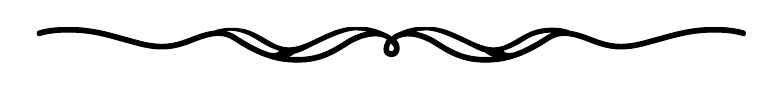
\begin{tikzpicture}
                  \node  (C) at (0,0) {};
                  \node (D) at (9,0) {};
                  \path (C) to [ornament=85] (D);
                \end{tikzpicture}}}}}%
  \end{center}%
}

\renewcommand{\labelitemii}{$\circ$}

\newcommand{\refbook}[1]{\small book: #1}
\newcommand{\refweb}[2]{\small web: \href{#2}{#1}}
